\documentclass[hyperref={colorlinks}]{beamer}

\usepackage{graphicx}
\usepackage{amsfonts,amsmath,color}       
\usepackage[spanish,activeacute]{babel}
\usepackage[utf 8x]{inputenc}
\usepackage{listings}
\usepackage{fancyvrb}
\lstset{basicstyle=\footnotesize\ttfamily,escapeinside={\%*}{*)}}

\usefonttheme{professionalfonts}
\usetheme{Darmstadt}
% Bergen, Boadilla, Copenhagen, Dresden, Hannover, Luebeck, AnnArbor, Berkeley, Darmstadt, Frankfurt, Ilmenau,     
% Madrid, Warsaw, Antibes, Berlin, CambridgeUS, Malmoe, PaloAlto
%\setBeamercovered{transparent}

\usepackage{minted} 
\usemintedstyle{emacs}

\begin{document}



\title[\LaTeX]{Introducci\'on a \LaTeX}
\author[G.R.]{{Guillermo F. Rubilar} \\ \tiny (Basado en el Tutorial de \LaTeX ,\\
por Juan Antonio Navarro P\'{e}rez, \\Universidad de las Am\'{e}ricas - Puebla)}
\frame{\titlepage}

%%%%%%%%%%%%%%%%%%%%%%%%%%%

\begin{frame}
\frametitle{Contenidos}
\tableofcontents
\end{frame}

%%%%%%%%%%%%%%%%%%%%%%%%%%%

\section{Introducci\'on}
\begin{frame}[fragile]\frametitle{?`\TeX{} y \LaTeX?}
\begin{itemize}
\item \TeX{} es un sistema profesional de \emph{composici'on tipogr'afica} desarrollado
por \href{http://www-cs-faculty.stanford.edu/~knuth}{Donald E. Knuth} (1977, Stanford).
\item \TeX{} fue dise\~nado para producir documentos (especialmente con expresiones matem'aticas) con la m'as alta \emph{calidad de imprenta}.
\item \LaTeX\ es un \emph{sistema de macros}, desarrollado sobre \TeX{} por \href{https://es.wikipedia.org/wiki/Leslie_Lamport}{Leslie Lamport} (1980's), para facilitar su uso por parte de los autores.
\end{itemize}
\end{frame}

\begin{frame}[fragile]\frametitle{?`\TeX{} y \LaTeX?}
\begin{itemize}
\item Michael Spivak desarrolla ams-TeX, ahora incorporado en \LaTeX\ como \texttt{amsmath} 
(1980's).
  \item \LaTeX\ 2.09 se transforma en \LaTeX2e (1990's).
  \item El proyecto \LaTeX\ 3. 
	\begin{center}
		
\includegraphics[width=6cm]{figs/tux26.pdf}
	\end{center}
\end{itemize}
\end{frame}


%\begin{frame}[fragile]\frametitle{Sistema de imprenta}
%\vspace{1.6cm}
%\begin{center}
%	\scalebox{0.8}{\input{imprenta.tex}}
%\end{center}
%\end{frame}


\begin{frame}[fragile]\frametitle{Word/Writer vs \LaTeX}
\begin{center}
\begin{tabular}{p{0.4\textwidth}p{0.4\textwidth}}
\multicolumn{1}{c}{Word/Writer	}     & \multicolumn{1}{c}{\LaTeX}      \\
\\

$\bullet$ WYSIWYG            & $\bullet$ Preprocesado          \\
$\bullet$ Muy f'acil de usar & $\bullet$ No siempre f'acil     \\
$\bullet$ Facilidades para insertar objetos 
                             & $\bullet$ Limitaciones por formatos de archivo \\[1ex]
$\bullet$ Lento y malo para tratar f'ormulas
                             & $\bullet$ Muy bueno para f'ormulas \\
$\bullet$ 'Enfasis en Dise\~no & $\bullet$ En Contenido         
\end{tabular}
\end{center}
\end{frame}

\begin{frame}[fragile]\frametitle{?`Por qu'e usar \LaTeX?}
\begin{itemize}
\item Produce documentos con calidad de imprenta.
\item Es utilizado por editoriales (Springer, Elsevier, \dots), revistas y congresos especializados.
\item Es una herramienta indispensable para f'isic@s, geof'isic@s, astr'onom@s, matem'atic@s, etc. y especialmente para investigador@s.
\item Es la mejor opci'on para escribir su \emph{tesis}!.
\end{itemize}
\end{frame}


\begin{frame}[fragile]\frametitle{Filosof'ia de \LaTeX}

\bigskip

\bigskip
\begin{block}{}
La persona que escribe debe de preocuparse del \textit{contenido} de sus documentos, y no (directamente) de la \textit{apariencia} que 'estos tendr'an en el resultado final.
\end{block}
\end{frame}

\section{Edici\'on B\'asica}


\begin{frame}[fragile]\frametitle{Mi primer documento}
\begin{block}{}
\begin{minted}{tex}
\documentclass{article}
\author{Nombre de Autor(a)}
\title{Mi Primer Documento}

\begin{document}
\maketitle

Hola. Este es mi primer documento.
\end{document}
\end{minted}
\end{block}
\end{frame}

%\begin{frame}[fragile]\frametitle{Proceso de compilaci'on}
%\vspace{0.6cm}
%\begin{center}
%	\scalebox{0.8}{\input{compilado.tex}}
%\end{center}
%\end{frame}

%\begin{frame}[fragile]\frametitle{Obtenci'on de PDF}
%\vspace{0.6cm}
%\begin{center}
%	\scalebox{0.8}{\input{compilado2.tex}}
%\end{center}
%\end{frame}

\begin{frame}[fragile]\frametitle{Proceso de compilaci'on}

\begin{block}{Forma tradicional}
\begin{itemize}
\item Compilar: \par
\texttt{> latex archivo.tex}
%\item Pre-visualizar: \par
%\texttt{> xdvi archivo.dvi}
%\item Generar Post-Script: \par
%\texttt{> dvips archivo.dvi -o archivo.ps}
%\item Imprimir: \par
%\texttt{> lpr -Plaser1sala4 archivo.ps}
\item Convertir archivo .dvi a Pdf: \par
\texttt{> dvipdf archivo.dvi}\par
%\texttt{> ps2pdf archivo.ps archivo.pdf}
\end{itemize}
\end{block}
\begin{block}{Forma r'apida (Recomendada)}
\begin{itemize}
\item Compilar directamente a pdf: \par
\texttt{> pdflatex archivo.tex}
\end{itemize}
\end{block}
\end{frame}


\begin{frame}[fragile]\frametitle{Clases de documentos}
Clases est'andares
\begin{itemize}
  \item \texttt{article} -- Art'iculo.
  \item \texttt{report} -- Reporte.
  \item \texttt{book} -- Libro.
  \item \texttt{letter} -- Cartas.
\end{itemize}
Clases extras
\begin{itemize}
  \item \texttt{beamer} -- Presentaciones.
  \item \texttt{prosper} -- Presentaciones.
  \item \texttt{poster} -- Poster.
\end{itemize}
\end{frame}

\begin{frame}[fragile]\frametitle{Unidades estructurales}
Para libros y reportes:
\begin{itemize}
  \item \verb|\part{...}|
  \item \verb|\chapter{...}|
\end{itemize}
Para libros, art'iculos y reportes:
\begin{itemize}
  \item \verb|\section{...}|
  \item \verb|\subsection{...}|
  \item \verb|\subsubsection{...}|
\end{itemize}
'Indice: \verb|\tableofcontents|.
\end{frame}

\begin{frame}[fragile]\frametitle{Listas con Vi\~netas}
\begin{block}{}
\begin{minted}{tex}
  \begin{itemize}
    \item Un elemento de la lista.
    \item Otro elemento de la lista.
  \end{itemize}
 \end{minted}
\end{block}
  
    \begin{itemize}
    \item Un elemento de la lista.
    \item Otro elemento de la lista.
  \end{itemize}
\end{frame}

\begin{frame}[fragile]\frametitle{Listas Enumeradas}
\begin{block}{}
\begin{minted}{tex}
  \begin{enumerate}
    \item El primer elemento de la lista.
    \item El segundo elemento de la lista.
  \end{enumerate}
 \end{minted}
\end{block}
  
   \begin{enumerate}
    \item El primer elemento de la lista.
    \item El segundo elemento de la lista.
  \end{enumerate}
\end{frame}

\begin{frame}[fragile]\frametitle{Listas Anidadas}
  \begin{enumerate}
    \item El primer elemento de la lista.
    \begin{enumerate}
      \item Un sub elemento.
      \item El segundo sub elemento.
    \end{enumerate}
    \item El segundo elemento de la lista.
    \begin{itemize}
      \item Con algunos puntos \dots
      \item \dots importantes.
    \end{itemize}
    \item Y el \'ultimo elemento.
  \end{enumerate}
\end{frame}

\begin{frame}[fragile]\frametitle{Listas Anidadas}
\begin{block}{}
\begin{minted}{tex}
  \begin{enumerate}
    \item El primer elemento de la lista.
    \begin{enumerate}
      \item Un sub elemento.
      \item El segundo sub elemento.
    \end{enumerate}
    \item El segundo elemento de la lista.
    \begin{itemize}
      \item Con algunos puntos \dots
      \item \dots importantes.
    \end{itemize}
    \item Y el \'ultimo elemento.
  \end{enumerate}
\end{minted}
\end{block}
\end{frame}

\begin{frame}[fragile]\frametitle{Citas Textuales}
\dots como la princesa dijo:
\begin{quote}
``Gracias por rescatarme. Pero la verdadera princesa est\'a en otro castillo.''
\end{quote}
Y ten\'ias que avanzar a otro castillo.

\begin{block}{}
\begin{minted}{tex}
\dots como la princesa dijo:
\begin{quote}
``Gracias por rescatarme. Pero la verdadera princesa
est\'a en otro castillo.''
\end{quote}
Y ten\'ias que avanzar a otro castillo.
\end{minted}
\end{block}
\end{frame}


\begin{frame}[fragile]\frametitle{Texto Enfatizado}

Decimos que un n\'umero es \emph{racional} si existen dos enteros \dots

\begin{block}{}
\begin{minted}{tex}
Decimos que un n\'umero es \emph{racional} si existen 
dos enteros \dots
\end{minted}
\end{block}

\begin{itemize}
\item \verb|\emph{...}| enfatiza parte del texto.
\item \emph{!`Piensa en contenido, no en formato!}
%\item Los t'erminos nuevos en definiciones usualmente se enfatizan.
\end{itemize}
\end{frame}


\begin{frame}[fragile]\frametitle{Notas al pie de p\'agina}
\begin{block}{}
\begin{minted}{tex}
Uno de los grandes personajes de la F\'isica sin duda 
es Sir Isaac Newton\footnote{Isaac Newton: 25 de 
diciembre de 1642 (jul.) / 4 de enero de 1643 (greg) 
-- 20 de marzo (jul.) / 31 de marzo de 1727 (greg.) 
fue un f\'isico, fil\'osofo, te\'ologo, inventor, 
alquimista y matem\'atico ingl\'es.} quien, entre 
otras cosas, desarroll\'o los fundamentos de la 
\emph{Mec\'anica}.
\end{minted}
\end{block}

Uno de los grandes personajes de la F\'isica sin duda es 
Sir Isaac Newton\footnote{Isaac Newton: 25 de diciembre de 
1642 (jul.) / 4 de enero de 1643 (greg) -- 20 de marzo 
(jul.) / 31 de marzo de 1727 (greg.) fue un f\'isico, 
fil\'osofo, te\'ologo, inventor, alquimista y matem\'atico 
ingl\'es.} quien, entre otras cosas, desarroll\'o los 
fundamentos de la \emph{Mec\'anica}.
\end{frame}


\begin{frame}[fragile]\frametitle{Comandos de Formato}

\begin{center}
\begin{tabular}{ll}
\verb|\textrm{}|  & \textrm{Romano} \\
\verb|\textsf{}|  & \textsf{Serif} \\
\verb|\texttt{}|  & \texttt{Typewriter} \\
\verb|\textbf{}|  & \textbf{Negritas} \\
\verb|\textit{}|   & \textit{It'alicas} \\
\verb|\textsl{}|   & \textsl{Slanted} \\
\verb|\textsc{}|  & \textsc{Small Caps} \\
\verb|\underline{}|  & \underline{Subrayado} \\
\end{tabular}
\end{center}

Hay versiones \verb|\mathXX{}| equivalentes para modo matem'atico.
Y \verb|\mathcal{}| $\mathcal{CAL}$.
\end{frame}

\begin{frame}[fragile]\frametitle{Tama\~no de Letra}
\begin{center}
\begin{tabular}{ll}
\verb|{\tiny }| & {\tiny Peque\~nita} \\
\verb|{\scriptsize}| & {\scriptsize scriptsize}\\
\verb|{\footnotesize}| & {\footnotesize tama\~no de nota al pie}\\
\verb|{\small }| & {\small Peque\~na} \\
\verb|{\normalsize }| & {\normalsize Normal} \\
\verb|{\large }| & {\large Grande} \\
\verb|{\Large }| & {\Large Grandota} \\
\verb|{\LARGE }| & {\LARGE Grandototota} \\
\verb|{\huge }| & {\huge Enorme} \\
\verb|{\Huge }| & {\Huge Mega Enorme} \\
\end{tabular}
\end{center}
\end{frame}

\begin{frame}[fragile]\frametitle{Comandos de Alineaci'on}
\begin{itemize}
\item \verb|\begin{center}| \par \verb|\end{center}|
\item \verb|\begin{flushleft}| \par \verb|\end{flushleft}|
\item \verb|\begin{flushright}| \par \verb|\end{flushright}|
\item \verb|\begin{sloppypar}| \par \verb|\end{sloppypar}|
\end{itemize}
\end{frame}

\begin{frame}[fragile]\frametitle{Espa\~nol y \LaTeX}
Forma tradicional
  \begin{center}
  \begin{tabular}{cc}
     Input      &   Resultado \\
     \verb+\'o+  &   'o       \\
     \verb+\'u+  &   'u       \\
     \verb+\'a+  &   'a       \\
     \verb+\'i+  &   'i        \\
     \verb+\~n+  &   \~n     \\
     \verb+\~N+  &   \~N     \\
     \verb+?`+  &   ?`     \\
     \verb+!`+  &   !`  
  \end{tabular}
\end{center}
\end{frame}


\begin{frame}[fragile]\frametitle{Espa\~nol y \LaTeX}
\verb|\usepackage[spanish, activeacute]{babel}|
  \begin{center}
  \begin{tabular}{cc}
     Input      &   Resultado \\
     \verb+'o+  &   'o       \\
     \verb+'u+  &   'u       \\
     \verb+'a+  &   'a       \\
     \verb+'i+  &   'i        \\
     \verb+~n+  &   \~n     \\
     \verb+'N+  &   'N     \\
     \verb+?`+  &   ?`     \\
     \verb+!`+  &   !`  
  \end{tabular}
\end{center}
\end{frame}

\begin{frame}[fragile]\frametitle{Espa\~nol y \LaTeX}
\begin{itemize}
\item El pre'ambulo \verb|\usepackage[spanish,activeacute]{babel}| tambi'en se encarga de los cortes de palabras al final de las l'ineas (recomendado!).
\item \verb|\usepackage[latin1]{inputenc}|  permite ingresar los tildes directamente en el texto. (no lo recomiendo, si otros usuarios usan Windows!, problemas de codificaci\'on).
\end{itemize}

De ahora en adelante, supondremos que estamos usando \verb|\usepackage[spanish,activeacute]{babel}|
\end{frame}

\begin{frame}[fragile]\frametitle{Reglas generales de edici'on}
\begin{itemize}
\item Usar espacios para separar \emph{palabras}.
\item Un espacio vale igual que mil.
\item Los fines de l{\'\i}nea sencillos no valen.
\end{itemize}
\begin{itemize}
\item Usar l{\'\i}neas vac'ias para separar \emph{p'arrafos}.
\item Una l{\'\i}nea vac'ia vale igual que mil.
\end{itemize}
\begin{itemize}
\item El espaciado y las sangr'ias son trabajo de \LaTeX, y lo
  sabe hacer muy bien.
\item \emph{No forzar espacios ni cortes de l'inea.}
\end{itemize}
\end{frame}



\part{Matem'aticas con \LaTeX}

\begin{frame}[fragile]\frametitle{F'ormulas en l'inea}
Las f'ormulas en l'inea ocurren dentro de la secuencia natural de un p'arrafo.

\begin{block}{}
\begin{minted}{tex}
Sea $x$ un n'umero real en el intervalo $(0, 1)$. 
Observe tambi'en que $0 < x^2 < 1$.
\end{minted}
\end{block}

\begin{quote}
Sea $x$ un n'umero real en el intervalo $(0, 1)$. 
Observe tambi'en que $0 < x^{2} < 1$.
\end{quote}

\end{frame}

\begin{frame}[fragile]\frametitle{F'ormulas en l'inea}
\begin{itemize}
  \item Los signos \verb|$ $| indican el contenido matem'atico.
  \item Todo el contenido matem'atico (y s'olo el contenido matem'atico) debe ser marcado.
  \item No usar el contenido matem'atico para poner it'alicas.
  \item Y no usar comandos de formato para marcar contenido matem'atico.
  \item Pensar en el contenido, \emph{!`no en el formato!}.
\end{itemize}
\end{frame}


\begin{frame}[fragile]\frametitle{S'imbolos Especiales}
\begin{itemize}
  \item Letras griegas min'usculas
   \begin{center}
      \begin{tabular}{clcl}
        $\alpha$ & \verb+\alpha+ & $\theta$   & \verb+\theta+    \\
        $\beta$  & \verb+\beta+  & $\vartheta$& \verb+\vartheta+ \\
        \multicolumn{4}{c}{\ldots}                               \\
        $\lambda$& \verb+\lambda+& $\varsigma$& \verb+\varsigma+ 
      \end{tabular}
    \end{center}
   \item Legras griegas may'usculas
   \begin{center}
   \begin{tabular}{llcllcll}
   $\Gamma $ & \verb|\Gamma| & & $\Xi $ & \verb|\Xi| & &$\Phi $ & \verb|\Phi|  \\
$\Delta $ & \verb|\Delta| & & $\Pi $ & \verb|\Pi| & & $\Psi $ & \verb|\Psi|  \\
$\Theta $ & \verb|\Theta| & &$\Sigma $ & \verb|\Sigma| & & $\Omega $ & \verb|\Omega|  \\
$\Lambda $ & \verb|\Lambda| & & $\Upsilon $ & \verb|\Upsilon|  \\
  \end{tabular}
  \end{center}
  \end{itemize}
\end{frame}

\begin{frame}[fragile]\frametitle{S'imbolos Especiales}
\begin{itemize}
\item Operaciones binarias
      \begin{center}
       \begin{tabular}{clcl}
          $\pm$      & \verb+\pm+      &  $\mp$    & \verb+\mp+        \\
          $\cdot$    & \verb+\cdot+    &  $\bullet$& \verb+\bullet+    \\
          $\setminus$& \verb+\setminus+&  $\cap$   & \verb+\cap+
       \end{tabular}
    \end{center}
  \item Acentos matem'aticos
  \begin{center}
  \begin{tabular}{llcll}
   \verb|\hat a| & $\hat a$ & &\verb|\check a| & $\check a$ \\
 \verb|\tilde a| & $\tilde a$ & &\verb|\acute a| &  $\acute a$ \\
 \verb|\grave a| & $\grave a$ & & \verb|\dot a|  & $\dot a$ \\
 \verb|\ddot a|  & $\ddot a$  & & \verb|\breve a| & $\breve a$ \\
 \verb|\bar a|   & $\bar a$  & & \verb|\vec a|   & $\vec a$
 \end{tabular}
 \end{center}
 \end{itemize}
\end{frame}

\begin{frame}[fragile]\frametitle{S'imbolos Especiales}
\begin{itemize}
  \item S'imbolos diversos
   \begin{center}
  \begin{tabular}{llcll}
  $\aleph $ & \verb|\aleph| & & $\prime $& \verb|\prime| \\
$\forall $& \verb|\forall|  & & $\hbar $& \verb|\hbar| \\
$\emptyset $ & \verb|\emptyset| & & $\exists $& \verb|\exists|  \\
$\imath $ & \verb|\imath| & & $\nabla $& \verb|\nabla| \\
$\neg $& \verb|\neg|  & & $\jmath $& \verb|\jmath| \\
$\surd $& \verb|\surd| & & $\flat $& \verb|\flat| \\
$\ell $& \verb|\ell| & &$\top $& \verb|\top| \\
\end{tabular}
 \end{center}
  \end{itemize}
\end{frame}

\begin{frame}[fragile]\frametitle{S'imbolos Especiales}
\begin{center}
  	\begin{tabular}{llcll}
	$\natural $ & \verb|\natural| & & $\wp $& \verb|\wp| \\
	$\bot $ & \verb|\bot| & & $\sharp $& \verb|\sharp| \\
	$\Re $& \verb|\Re| & & $\Vert $& \verb.\|. \\
	$\clubsuit $& \verb|\clubsuit| & & $\Im $&\verb|\Im| \\
	$\diamondsuit $&  \verb|\diamondsuit| & & $\partial $& \verb|\partial| \\
	$\triangle $& \verb|\triangle| & & $\heartsuit $& \verb|\heartsuit| \\
	$\infty $& \verb|\infty| & & $\backslash $& \verb|\backslash| \\
	$\spadesuit $& \verb|\spadesuit| & & $\mho $& \verb|\mho| \\
	$\Box $& \verb|\Box| & &$\Diamond $& \verb|\Diamond| \\
	$\angle $ & \verb|\angle| && &\\
  	\end{tabular}
\end{center}
\end{frame}

\begin{frame}[fragile]\frametitle{S'imbolos Especiales}
  \begin{itemize}
   \item Nombres de funciones de uso com'un: \verb|\sin|, \verb|\cos|, \verb|\log|, \verb|\lim|, \dots
   \item Algunos comandos t'ipicos:
   
\begin{center}
  \begin{tabular}{ll}
    \verb|\sqrt{2}| & $\sqrt{2}$ \\
    \verb|x \leq 4| & $x \leq 4$ \\
    \verb|\frac{1}{3+i}| & $\frac{1}{3+i}$ \\
  \end{tabular}
\end{center}
	
	\item Caracteres especiales (reservados en \LaTeX): \verb|$ & % # _ ^ { } ~ \| se generan usando \verb+\$ \& \% \# \_ \verb|^| \{ \} \verb|~| y \verb|\|+
	
  \end{itemize}
\end{frame}

\begin{frame}[fragile]\frametitle{Exponentes y sub'indices}
\begin{itemize}
  \item Exponentes: \verb|x^2|: $x^2$
  \item Sub'indices: \verb|x_i|: $x_i$
  \item Para usar exponentes y sub'indices de m'as de un caracter, usar \verb|{}|. Ejemplos
  \begin{center}
  \begin{tabular}{ll}
    \verb|x^{2\pi}|      & $x^{2\pi}$ \\
    \verb|x_{i+1}|       & $x_{i+1}$ \\
    \verb|x_{i+1}^{2}|   & $x_{i+1}^{2}$ \\
    \verb|x_{(i+1)^{2}}| & $x_{(i+1)^{2}}$ \\
  \end{tabular}
  \end{center}
\end{itemize}
\end{frame}

\begin{frame}[fragile]\frametitle{L'imites y sumatorias}
\begin{itemize}
  \item Comandos: \verb|\lim|, \verb|\sum|, \verb|\int|
  \item Ejemplos:
\end{itemize}
  \begin{center}
  \begin{tabular}{ll}
    \verb|\lim_{x \to 0} \sin(x)/x|      & \quad $\lim_{x \to 0} \sin(x)/x$ \\[2pt]
    \verb|\sum_{i=0}^n i^{2}|          & \quad $\sum_{i=0}^{n} i^{2}$     \\[2pt]
    \verb|F(x) = \int_0^1 f(x)\,dx|  & \quad $F(x) = \int_{0}^{1} f(x)\,dx$ \\
  \end{tabular}
  \end{center}
\end{frame}

\begin{frame}[fragile]\frametitle{Entorno ``equation''}
\begin{block}{}
\begin{minted}{tex}
La suma de cuadrados
\begin{equation}
  \sum_{i=0}^n i^2
\end{equation}
tiene una f\'ormula muy sencilla.
\end{minted}
\end{block}

\begin{quote}
La suma de cuadrados
\begin{equation}
  \sum_{i=0}^{n} i^{2}
\end{equation}
tiene una f\'ormula muy sencilla.
\end{quote}
\end{frame}

\begin{frame}[fragile]\frametitle{Entorno ``equation''}
\begin{block}{}
\begin{minted}{tex}
\dots y despu\'es de muchos c\'alculos llegamos a la
inevitable conclusi\'on que 
\begin{equation}
  \lim_{x \to 0} \frac{\sin(x)}{x} = 1.
\end{equation}

Pasando a otros temas \dots
\end{minted}
\end{block}


\begin{quote}
\dots y despu\'es de muchos c\'alculos llegamos a la
inevitable conclusi\'on que 
\begin{equation}
  \lim_{x \to 0} \frac{\sin(x)}{x} = 1.
\end{equation}

Pasando a otros temas \dots
\end{quote}
\end{frame}

\begin{frame}[fragile]\frametitle{Notas de Redacci'on}
\begin{itemize}
  \item Las f'ormulas deben ocurrir de manera natural dentro de la lectura 
    de un p'arrafo (las ecuaciones se leen como parte del texto!).
%  \item Recuerda los signos de puntuaci'on. Utiliza los comandos 
%     \verb|\,,| o \verb|\,.| al final de una f'ormula en modo display si es necesario.
  \item No dejar l{\'\i}neas en blanco entre los comandos \verb|\begin{equation}|,
   \verb|\end{equation}| y el resto de las l'ineas del p'arrafo. Recuerda que la
   f'ormula \emph{forma parte} del p'arrafo.
\item \LaTeX numera autom'aticamente las ecuaciones!.
\item En ocasiones es conveniente agregar peque\~nos espacios:
	\begin{itemize}
		\item \verb|\,| espacio delgado: $\int f(x)\,dx$ (\verb|$\int f(x)\,dx$|).
		\item \verb|\;| espacio ancho: $\int f(x)\; dx$ (\verb|$\int f(x)\; dx$|).
		\item \verb|\ | espacio normal: $\int f(x)\ dx$ (\verb|$\int f(x)\  dx$|).
		\item \verb|\quad| espacio grande: $\int f(x)\quad dx$ (\verb|$\int f(x)\quad  dx$|).
		\item \verb|\qquad| espacio m'as grande: $\int f(x)\qquad dx$ (\verb|$\int f(x)\qquad  dx$|)
	\end{itemize}
\end{itemize}
\end{frame}



\begin{frame}[fragile]\frametitle{Arreglos y matrices}

\begin{block}{}
\begin{minted}{tex}
\begin{equation}
  \left(\begin{array}{ccc}
     \cos\theta & \sin\theta & 0 \\
    -\sin\theta & \cos\theta & 0 \\
     T_x       & T_y       & 1
  \end{array}\right)
\end{equation}
\end{minted}
\end{block}


\begin{equation}
  \left(\begin{array}{ccc}
     \cos\theta & \sin\theta & 0 \\
    -\sin\theta & \cos\theta & 0 \\
     T_x       & T_y       & 1
  \end{array}\right)
\end{equation}

\end{frame}

\begin{frame}[fragile]\frametitle{Arreglos y matrices}
\begin{itemize}
  \item Los comandos \verb|\left| y \verb|\right| ponen par'entesis grandes. Se pueden
    usar combinaciones de: \verb|(|, \verb|)|, \verb|[|, \verb|]|,
    \verb|\{|, \verb|\}|, \verb#|#, \verb|.|, \dots
  \item El ambiente \verb|array| recibe una lista de las columnas del arreglo,
     una letra: \verb|l| (left), \verb|c| (center), \verb|r| (right) para
     indicar la al{\'\i}neaci'on de cada columna.
  \item Las columnas se separan con \verb|&| y los renglones con \verb|\\|.
\end{itemize}
\end{frame}

\begin{frame}[fragile]\frametitle{Funciones por partes}
\begin{equation}
  f(x) = \left\{
    \begin{array}{ll}
      x      & 0 \leq x \leq 1 \\
      1 - x  & 1 \leq x \leq 2 \\
      0      & \text{en cualquier otro caso}
    \end{array}\right.
\end{equation}
\end{frame}

\begin{frame}[fragile]\frametitle{Funciones por partes}

\begin{block}{}
\begin{minted}{tex}
\usepackage{amsmath}
...
\begin{equation}
  f(x) = \left\{
    \begin{array}{ll}
      x      & 0 \leq x \leq 1 \\
      1 - x  & 1 \leq x \leq 2 \\
      0      & \text{en cualquier otro caso}
    \end{array}\right.
\end{equation}
\end{minted}
\end{block}

\begin{itemize}
  \item \verb|\right.| coloca un delimitador invisible (para usar \verb|\text|).
  \item No olvidar incluir el paquete \verb|amsmath|.
\end{itemize}
\end{frame}

%\begin{frame}[fragile]\frametitle{Ecuaciones muy largas}
%\begin{equation}
%  \begin{array}{rcl}
%    \Sigma & = & x_{1} + x_{2} + x_{3} + x_{4} + x_{5} + \\
%           &   & {} + x_{6} + x_{7} + x_{8} + x_{9} +    \\
%           &   & {} + x_{10} + x_{11} + x_{12} + x_{13}  \\
%           & = & \sum_{i=1}^{13} x_{i}
%  \end{array}
%\end{equation}
%
%\begin{verbatim}
%\begin{equation}
%	\begin{array}{rcl}
% 	 \Sigma & = & x_{1} + x_{2} + x_{3} + x_{4} + x_{5} + \\
%         &   & {} + x_{6} + x_{7} + x_{8} + x_{9} +    \\
%         &   & {} + x_{10} + x_{11} + x_{12} + x_{13}  \\
%         & = & \sum_{i=1}^{13} x_{i}
%	\end{array}
%\end{equation}
%\end{verbatim}
%\end{frame}

\begin{frame}[fragile]\frametitle{M\'ultiples ecuaciones alineadas}
\begin{eqnarray}
I &=&I_{cm}+MD^{2} \\
&=&\frac{1}{12}ML^2 +M\left( \frac{L}{2}-\frac{L}{5}\right)^2 \\
&=&\frac{13}{75}L^2 M \\
&\approx&9,7067\times 10^{-2} [kg\,m^2] .
\end{eqnarray}
\end{frame}

\begin{frame}[fragile]\frametitle{M\'ultiples ecuaciones alineadas}
\begin{block}{}
\begin{minted}{tex}
\usepackage{amsmath}
\begin{eqnarray}
   I &=&I_{cm}+MD^{2} \\
     &=&\frac{1}{12} ML^2 + M\left( \frac{L}{2}
     	-\frac{L}{5} \right)^2 \\
     &=&\frac{13}{75} L^{2} M \\
     &\approx & 9,7067 \times 10^{-2} [kg\,m^2].
\end{eqnarray}
\end{minted}
\end{block}
\end{frame}

\begin{frame}[fragile]\frametitle{M\'ultiples ecuaciones alineadas:  \texttt{align} de \texttt{amsmath}}
El paquete \texttt{amsmath} suministra el entorno \texttt{align}, con una sintaxis casi igual a \texttt{eqnarray}, pero con algunas mejoras en detalles de alineaci'on:
\begin{align}
I &= I_{cm} + MD^2 \\
&= \frac{1}{12} ML^2 + M\left(\frac{L}{2}-\frac{L}{5}\right)^2 \\
&= \frac{13}{75} L^2M \\
&\approx 9,7067 \times 10^{-2} [kg\,m^2].
\end{align}
\end{frame}

\begin{frame}[fragile]\frametitle{M\'ultiples ecuaciones alineadas:  \texttt{align} de \texttt{amsmath}}
\begin{block}{}
\begin{minted}{tex}
\begin{align}
I &= I_{cm} + MD^2 \\
&= \frac{1}{12} ML^2 + M\left(\frac{L}{2}
	-\frac{L}{5}\right)^2 \\
&= \frac{13}{75} L^2M \\
&\approx 9,7067 \times 10^{-2} [kg\,m^2].
\end{align}
\end{minted}
\end{block}
\end{frame}

\section{Referencias Cruzadas}

\begin{frame}[fragile]\frametitle{Referencias Cruzadas}
 El torque resultante es la suma del torque aplicado
sobre 1 m\'as el torque aplicado sobre 2. Es decir:
\begin{equation}
\tau_{total}=\tau_1+\tau_2,  \label{Ttotal}
\end{equation}
donde
\begin{equation}
\tau_1 =r_1 F_1 \sin\theta_1,  \label{T11}
\end{equation}
es positivo ya que la rotaci\'on va en sentido anti-horario, mientras que
\begin{equation}
\tau_2 = -r_2 F_2 \sin\theta_2,  \label{T22}
\end{equation}
es negativo ya que la rotaci\'on va en sentido horario. 
Luego, reemplazando (\ref{T11}) y (\ref{T22}) en (\ref{Ttotal}), 
tendremos que \dots
\end{frame}

\begin{frame}[fragile]%\frametitle{Referencias Cruzadas}
\begin{block}{}
\begin{minted}{tex}
 El torque resultante es la suma del torque aplicado
sobre 1 m\'as el torque aplicado sobre 2. Es decir:
\begin{equation}
\tau_{total}=\tau_1+\tau_2,  \label{Ttotal}
\end{equation}
donde
\begin{equation}
\tau_1 =r_1 F_1 \sin\theta_1,  \label{T11}
\end{equation}
es positivo ya que la rotaci\'on va en sentido 
anti-horario, mientras que
\begin{equation}
\tau_2 = -r_2 F_2 \sin\theta_2,  \label{T22}
\end{equation}
es negativo ya que la rotaci\'on va en sentido 
horario. Luego, reemplazando (\ref{T11}) y (\ref{T22}) 
en (\ref{Ttotal}), tendremos que \dots
\end{minted}
\end{block}
\end{frame}


\begin{frame}[fragile]\frametitle{Referencias Cruzadas}
\begin{itemize}
\item Se puede poner \verb|\label{..}| despu'es de:
  \begin{itemize}
    \item \verb|\begin{equation}|, \verb|\begin{eqnarray}|, \dots
    \item \verb|\begin{table}|, \verb|\begin{figure}|, \dots
    \item \verb|\chapter{..}|, \verb|\section{..}|, \dots
    \item Casi cualquier cosa que numere.
  \end{itemize}
\item Se puede poner \verb|\ref{..}|:
  \begin{itemize}
    \item !`Donde quieras en el documento!
  \end{itemize}
\item Recuerda recompilar para actualizar referencias.
\item \texttt{amsmath} tambi'en suministra \verb|\eqref{..}| para citar ecuaciones, que permite reemplazar \verb|(\ref{..})| por \verb|\eqref{..}|.
\end{itemize}
\end{frame}

\begin{frame}[fragile]\frametitle{Consejos de Redacci\'on}
  \begin{itemize}
%  \item Notaci'on: \verb|Cap\'itulo~\ref{intro}|
%  \begin{itemize}
%    \item La palabra clave en may'uscula.
%    \item No olvides usar `\verb|~|'{} en lugar de espacio.
%  \end{itemize}
  \item Usa nombres descriptivos para las etiquetas:
  \begin{itemize}
    \item \texttt{newton}, \texttt{maxwellhom}, \texttt{solucion2}
  \end{itemize}
  \item Evita usar nombres que no te dicen nada:
  \begin{itemize}
    \item \texttt{tdmapmu}, \texttt{ec2}, \texttt{p}
  \end{itemize}
\end{itemize}
\end{frame}



\begin{frame}[fragile]\frametitle{Citas Bibliogr\'aficas}
\begin{block}{}
\begin{minted}{tex}
\begin{document}
...

Si Ud. quiere ser sec@ en Relatividad General, 
l\'ease este librito \cite{MTW73}.

...

\begin{thebibliography}{99}
\bibitem{MTW73} C.W. Misner, K.S. Thorne and J.A. 
Wheleer, {\em Gravitation},  W.H. Freeman and Company, 
San Francisco (1973).
\end{thebibliography}
\end{document}
\end{minted}
\end{block}
\end{frame}

\part{Tablas y Figuras}
\section{Tablas y Figuras}

\begin{frame}[fragile]\frametitle{Tablas Simples}

\begin{center}
\begin{tabular}{c|cc}
A\~no  & Ventas   & Inversi\'on \\ \hline
1999  & \$ 3.900 &    1.4\%   \\
2000  & \$ 2.700 &    3.6\%   \\
2001  & \$ 3.200 &    2.3\%   \\
2002  & \$ 3.700 &    4.9\%   \\
2003  & \$ 4.100 &    3.4\%   \\
\end{tabular}
\end{center}

\end{frame}

\begin{frame}[fragile]\frametitle{Tablas Simples}
\begin{block}{}
\begin{minted}{tex}
\begin{center}
  \begin{tabular}{c|cc}
    A\~no  & Ventas   & Inversi\'on \\ \hline
    1999  & \$ 3.900 &    1.4\%   \\
    2000  & \$ 2.700 &    3.6\%   \\
    2001  & \$ 3.200 &    2.3\%   \\
    2002  & \$ 3.700 &    4.9\%   \\
    2003  & \$ 4.100 &    3.4\%   \\
  \end{tabular}
\end{center}
\end{minted}
\end{block}
\end{frame}

\begin{frame}[fragile]\frametitle{Tablas Simples}
\begin{itemize}
  \item El ambiente \verb|tabular| se parece mucho a \verb|array|, pero funciona
    en modo texto.
  \item Usa barras \verb$|$ en la descripci'on de la columna para indicar lineas
    verticales, y el comando \verb|\hline| para l'ineas horizontales.
  \item \textbf{Sugerencia}: No agreges demasiadas l'ineas a una tabla, usa s'olo las 
    necesarias para separar o distinguir los valores importantes.
\end{itemize}
\end{frame}

\begin{frame}[fragile]\frametitle{Multicolumnas}
\begin{center}
  \begin{tabular}{cc|cc}
    \multicolumn{2}{c|}{Originales} & \multicolumn{2}{c}{Transformados} \\
      $x$ & $y$ & $x$ & $y$ \\ \hline
      0.0 & 0.0 & 0.5 & 0.5 \\ 
      4.0 & 7.0 & 2.0 & 3.5 \\ 
      5.0 & 3.0 & 2.5 & 1.5 \\ 
      3.0 & 5.0 & 1.5 & 2.5 \\ 
  \end{tabular}
\end{center}
\end{frame}

\begin{frame}[fragile]\frametitle{Multicolumnas}
\begin{block}{}
\begin{minted}{tex}
\begin{center}
  \begin{tabular}{cc|cc}
    \multicolumn{2}{c|}{Originales} & 
         \multicolumn{2}{c}{Transformados} \\
      $x$ & $y$ & $x$ & $y$ \\ \hline
      0.0 & 0.0 & 0.5 & 0.5 \\ 
      4.0 & 7.0 & 2.0 & 3.5 \\ 
      5.0 & 3.0 & 2.5 & 1.5 \\ 
      3.0 & 5.0 & 1.5 & 2.5 \\ 
  \end{tabular}
\end{center}
\end{minted}
\end{block}
\end{frame}

\begin{frame}[fragile]\frametitle{Elementos Flotantes}
En \LaTeX existen diversos tipos de \textbf{elemento flotantes}, cuya posición en el documento final es decidida al momento de compilar: tablas y figuras
\begin{table}
	\begin{center}
    \begin{tabular}{c|cc}
      A\~no  & Ventas   & Inversi'on \\ \hline
      1999  & \$ 3.900 &    1.4\%   \\
      2000  & \$ 2.700 &    3.6\%   \\
      2001  & \$ 3.200 &    2.3\%   \\
      2002  & \$ 3.700 &    4.9\%   \\
      2003  & \$ 4.100 &    3.4\%   \\
    \end{tabular}
	\end{center}

	\caption{Ventas Empresa Pato Feliz}
	\label{tab:ventaspatofeliz}
\end{table}
\end{frame}

\begin{frame}[fragile]\frametitle{Elementos Flotantes}
\begin{block}{}
\begin{minted}{tex}
\begin{table}
  \begin{center}
    \begin{tabular}{c|cc}
      ...
    \end{tabular}
  \end{center}

  \caption{Ventas Empresa Pato Feliz}
  \label{tab:ventaspatofeliz}
\end{table}
\end{minted}
\end{block}
\end{frame}

\begin{frame}[fragile]\frametitle{Elementos Flotantes}
\begin{itemize}
  \item \LaTeX\ tratar'a de acomodar los elementos flotantes lo mejor que
    pueda en las p'aginas cercanas al c'odigo de la tabla.
  \item No tratar de forzar la posici'on de la tabla en el documento.
    \underline{Dejar que \LaTeX\ haga su trabajo}.
  \item Utilizar \verb|\ref{..}| y \verb|\label{..}| para hacer referencia a la
    tabla. Evitar redacciones del tipo: ``\dots en el cuadro siguiente:''
\end{itemize}
\end{frame}

\begin{frame}[fragile]\frametitle{Insertar Figuras}
\begin{figure}
	\begin{center}
		\includegraphics[width=5cm]{figs/3cuerdas.pdf}
	\end{center}
	\caption{Un bloque sostenido por tres cuerdas.}
	\label{fig:3cuerdas}
\end{figure}

\end{frame}

\begin{frame}[fragile]\frametitle{Insertar Figuras}
\begin{block}{}
\begin{minted}{tex}
\usepackage{graphicx}

...

\begin{figure}
  \begin{center}
    \includegraphics[width=5cm]{3cuerdas.pdf}
  \end{center}
  \caption{Un bloque sostenido por tres cuerdas.}
  \label{fig:3cuerdas}
\end{figure}
\end{minted}
\end{block}
\end{frame}

\begin{frame}[fragile]\frametitle{Insertar Figuras}
\begin{itemize}
  \item (Cuando se generan archivos \texttt{.ps} (compilando con \texttt{latex}) se pueden insertar im'agenes en formato \texttt{.eps}, \texttt{.ps}.)
  \item Cuando se generan archivos \texttt{.pdf} (compilando con \texttt{pdflatex}) se pueden insertar im'agenes en formato \texttt{.jpg}, \texttt{.png}, \texttt{.pdf}.
  \item Recomiendo Inkscape, Python, LibreOffice  para crear gr'aficos vectoriales (.svg, .ps, .eps, .pdf); Gimp para fotos (.png, .jpg).
\end{itemize}
\end{frame}

\begin{frame}[fragile]\frametitle{Insertar Figuras}
\begin{itemize}
\item La opci'on  \verb|[width=6cm]| se puede usar para modificar el ancho
  tama\~no de una imagen. Tambi'en existe la opci'on \texttt{height}, p.ej. \verb|[height=5cm]|.
\item Tambi'en puede usarse la opci'on \verb|[scale=0.6]| para re-escalar la figura.
\begin{verbatim}
	\includegraphics[scale=0.6]{transistor.pdf}
\end{verbatim}  
\end{itemize}
\end{frame}

\begin{frame}[fragile]\frametitle{'Indices}

\begin{itemize}
\item Los comandos \verb|\listoffigures| y \verb|\listoftables| generan
los 'indices de figuras y tablas respectivamente.
\item En los 'indices se agregan s'olo las figuras y tablas que hayas agregado como
elementos flotantes.
\end{itemize}
\end{frame}


%
%\part{Definir nuevas macros}
%
%\begin{frame}[fragile]\frametitle{Nuevos Comandos}
%
%\begin{itemize}
%\item La instrucci'on 
%\begin{center}
%\verb|\newcommand{|\textit{comando}\verb|}{|\textit{definici'on}\verb|}|
%\end{center}
%se utiliza para definir nuevos comandos.
%\end{itemize}
%
%\begin{verbatim}
%\newcommand{\RR}{{\mathbb R}}    % Conjunto de los Reales
%\newcommand{\QQ}{{\mathbb Q}}    % Conjunto de los Racionales
%\newcommand{\tq}{\;|\;}
%\newcommand{\prove}{\vdash}
%\end{verbatim}
%\end{frame}
%
%\begin{frame}[fragile]\frametitle{Nuevos Comandos}
%\begin{itemize}
%\item Puedes tambi'en definir nuevos comandos con argumentos
%\begin{verbatim}[escapechar=\$]
%\newcommand{\set}[1]{\left\{#1\right\}}
%\newcommand{\iprod}[2]{\left\langle #1, #2 \right\rangle}
%\newcommand{\logic}[1]{\ensuremath{\mathrm{#1}}}
%\newcommand{\provein}[1]{\prove_\logic{#1}}
%\end{verbatim}
%\item El n'umero entre corchetes indica el n'umero de argumentos, y haces referencia
%a ellos con los comandos \verb|#1|, \verb|#2|, etc.
%\end{itemize}
%\end{frame}
%
%


\end{document}